\documentclass[12pt,a4paper, spanish]{report}
\usepackage[spanish]{babel}
\usepackage[latin1]{inputenc}  % Ambos para solucin de asuntos de idioma
\usepackage[T1]{fontenc}
\usepackage{tocbibind}  % Bibliografa en el indice
\usepackage{titlesec}  % Posibilidad de editar los formatos de chapter y section
%\usepackage{times}  % Fuente de letras
\usepackage{amsmath,amssymb,mathrsfs,mathptmx}  % Matemticas varias
\usepackage{hyperref} % Para escribir URLs



% --- Arreglos varios para la inclusion de imgenes
%\usepackage[pdftex]{graphicx}
%\usepackage[dvips]{graphicx}
\usepackage{graphicx}
\usepackage{epstopdf}
\usepackage{float}
\usepackage{subfigure}
%\usepackage{subfig}
\usepackage{wrapfig}
\usepackage[usenames,dvipsnames]{color}
\DeclareGraphicsExtensions{.png,.jpg,.pdf,.mps,.gif,.bmp, .eps}


	

\usepackage{multirow}
\usepackage{multicol}
\usepackage{tabulary}
\usepackage[table]{xcolor}
\usepackage{color}
\usepackage{listings}
%\usepackage{subfloat}
\usepackage{tikz}

\setcounter{secnumdepth}{3}
\setcounter{tocdepth}{3}


% --- Para las dimensiones de los mrgenes etc
\frenchspacing \addtolength{\hoffset}{-1.5cm}
\addtolength{\textwidth}{3cm} \addtolength{\voffset}{-2.5cm}
\addtolength{\textheight}{4cm}
% --- Para el encabezado
\usepackage{fancyhdr}
\fancyhead[R]{2012}\fancyhead[L]{enCuadro} \fancyfoot[C]{\thepage}
\pagestyle{fancy}

% --- Formato de la etiqueta Chapter
%\newcommand{\bigrule}{\titlerule[0.5mm]}
%\titleformat{\chapter}[display]{\bfseries\Huge}
%{\Large\chaptertitlename\ \Large\thechapter}
%{0mm} {\filleft} [\vspace{0.5mm} \bigrule]

\titleformat{\chapter}[display]
{\normalfont\Large\filcenter}
{\titlerule[1pt]%
\vspace{1pt}%
\titlerule
\vspace{1pc}%
\LARGE\MakeUppercase{\chaptertitlename} \thechapter}
{1pc}
{\titlerule
\vspace{1pc}%
\Huge}

%-------------------------

\begin{document}
% Esto es para que se muestren todas las referencias aunque no se citen:
\nocite{*}

\renewcommand{\tablename}{Tabla}
\renewcommand{\theenumi}{\Roman{enumi}}
\renewcommand{\labelenumi}{[\textbf{\theenumi}]}
\renewcommand{\thefootnote}{\arabic{footnote}}
% --- Modificacin de entornos enumerate
\renewcommand{\theenumi}{\roman{enumi}}
\renewcommand{\labelenumi}{\theenumi)}
% --- Modificacin de entornos enumerate

% --- Para hacer highlights
\newcommand{\highlAmarillo}[1]{\colorbox{yellow}{#1}}
\newcommand{\highlVerde}[1]{\colorbox{green}{#1}}
\newcommand{\highlRojo}[1]{\colorbox{red}{#1}}

%
\tableofcontents


\chapter{Alcance del proyecto}
\label{chap: alcance}
\section{Introducci�n}

En el presente cap�tulo se habla del alcance del proyecto. Esto es, se plantean los objetivos tal y como fueron formulados originalmente y luego se los clasifica en las tres partes fundamentales del proyecto: \textit{investigaci�n}, \textit{implementaci�n} y \textit{aplicaci�n}. Estas son ponderadas en funci�n de la importancia que tienen en el mismo, as� como las dedicaci�n total que se les dio. Luego, se resume la estructura de lo que termin� siendo la aplicaci�n final, de manera de poder comprender a todo el proyecto en su conjunto. Finalmente, se comenta en qu� parte de la documentaci�n se detalla cada parte de dicha estructura.\\
 
\section{Objetivos del proyecto}

El presente proyecto de fin de carrera cuenta con varios objetivos en conjunto. Por un lado, se busca investigar distintos algoritmos de procesamiento de im�genes con el fin de implementarlos y estudiar su desempe\~no sobre ciertas plataformas m�viles; para lo cual tambi�n se deben estudiar dichas plataformas y elegir la m�s apta de entre las opciones \textit{Android} e \textit{iOS}. Por otro lado, m�s adelante en el proyecto, se espera utilizar lo investigado para lograr una aplicaci�n de realidad aumentada completa funcionando sobre un dispositivo m�vil y en tiempo real. Finalmente se le quiere dar, a la aplicaci�n de realidad aumentada, un marco dentro de un \textit{recorrido interactivo en realidad aumentada} para museos.\\

Los objetivos anteriores pueden resumirse en las tres partes fundamentales del proyecto, que se expresan a continuaci�n:

\begin{itemize}
\item[1.] \textbf{Investigaci�n:} comprensi�n de la arquitectura de las plataformas m�viles y de sus plataformas de desarrollo, con el objetivo de embeber los distintos algoritmos y \textit{software} en general en las mismas. Estudio de las diferentes maneras de lograr la realidad aumentada, elecci�n de los algoritmos a utilizar, su comprensi�n y en algunos casos su implementaci�n total o parcial. Aprendizaje de herramientas en general.
\item[2.] \textbf{Implementaci�n}: integraci�n de los distintos bloques para lograr la realidad aumentada. Implementaci�n de bloques l�gicos accesorios que faciliten la integraci�n de los primeros. Validaci�n de los algoritmos utilizados y desarrollados.
\item[3.] \textbf{Aplicaci�n}: implementaci�n de una aplicaci�n total en la que el usuario ingrese al museo, se ubique dentro de �l, se dirija a un cuadro, reciba informaci�n respecto del mismo y finalmente disfrute de la realidad aumentada sobre la obra.
\end{itemize}

Cada una de ellas se jerarquiz� en funci�n de la importancia que se que cree tiene para el proyecto, as� como tambi�n el tiempo que se les dedic�:\\

$$
\begin{array}{|c|c|} \hline
\textbf{Frente de trabajo}			& \textbf{Porcentaje} \\ \hline
\small \textbf{Investigaci�n}		&	50\% \\ \hline
\small \textbf{Implementaci�n}	& 30\% \\ \hline
\small \textbf{Aplicaci�n}			& 20\%  \\ \hline
\end{array}
$$

Es importante aclarar que en ocasiones el l�mite entre los tres frentes de trabajo es difuso.\\

\section{Estado del arte}
Para llevar a cabo los objetivos planteados es bueno tener un contexto del estado del arte en cuanto al desarrollo de aplicaciones de realidad aumentada. Existen en la actualidad m\'ultiples kits de desarrollo comerciales para aplicaciones de realidad aumentada, en los que de manera sencilla, se logran este tipo de aplicaciones con desempe\~nos verdaderamente muy buenos. Tal es el caso de \textit{Metaio} \cite{metaio12}, \textit{Vuforia} \cite{vuforia12}, \textit{String} \cite{string12} y \textit{Aurasma} \cite{aurasma12}. Por su parte, \textit{Layar} \cite{layar12}, es tambi\'en un kit de desarrollo para aplicaciones de realidad aumentada, pero se especializa en el agregado de contenido digital s\'olo sobre p�ginas impresas como revistas y cat�logos. Ninguna de las herramientas anteriores es gratuita y ni siquiera en c\'odigo abierto. En la Figura \ref{fig: metaioystring} se muestra un ejemplo que incluye por defecto \textit{Metaio} y otro que incluye \textit{String}.\\

\begin{figure}[H]
\centering
$$
\begin{array}{cc}
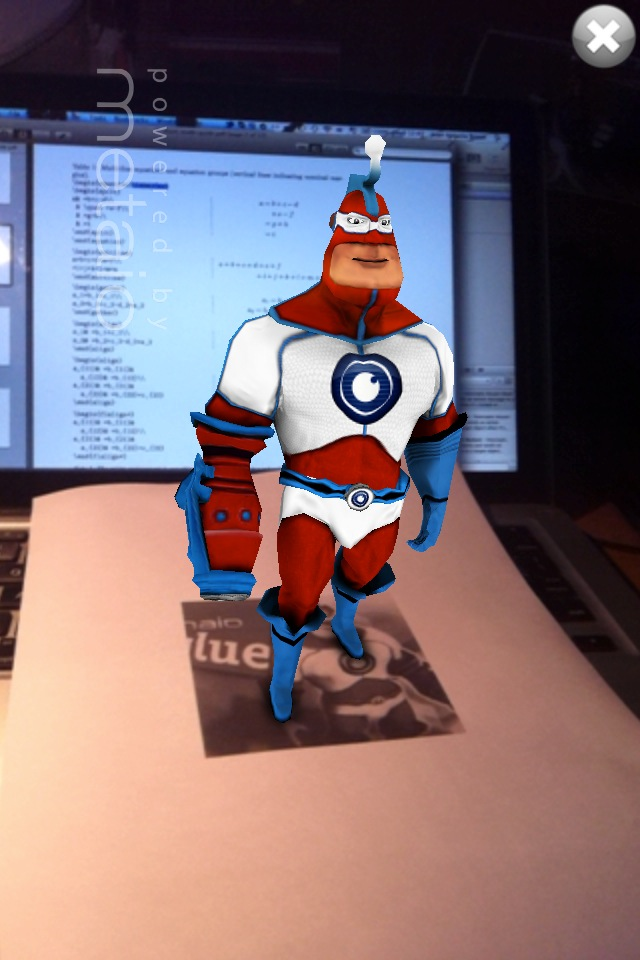
\includegraphics[scale=0.222]{figs_alcance/metaio.png} & 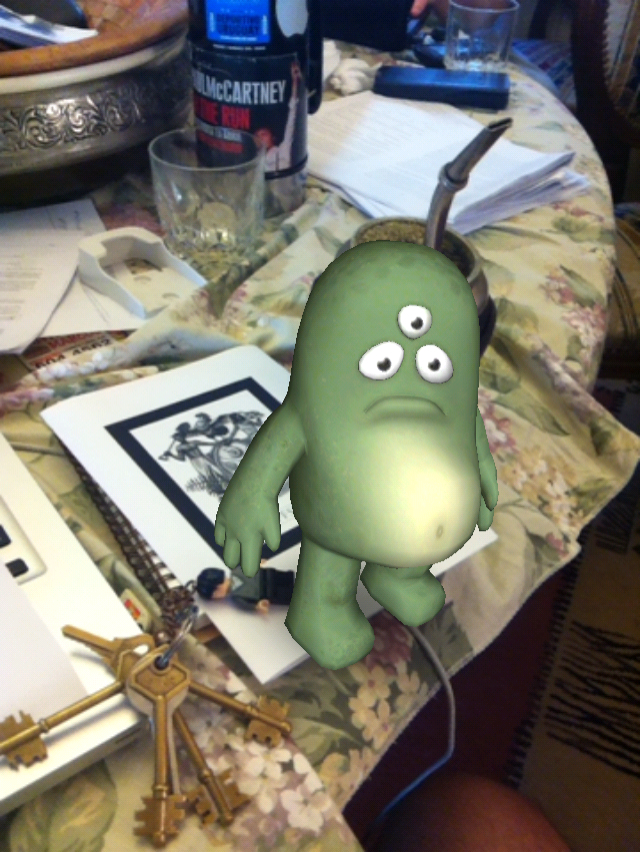
\includegraphics[scale=0.5]{figs_alcance/string.png}
\end{array}
$$
\caption{Izq.: Ejemplo de realidad aumentada que incluye por defecto el kit de desarrollo \textit{Metaio}. Der.: Otro ejemplo de realidad aumentada inclu�do por \textit{String}.}
\label{fig: metaioystring}
\end{figure}

Si bien se probaron algunas de estas herramientas y se tomaron de ellas est\'andares en cuanto a la \textit{performance} que una aplicaci\'on de realidad aumentada debe tener, \textbf{no es un objetivo} del proyecto el desarrollo de aplicaciones de realidad aumentada con kits de desarrollo ya existentes. Se hace hincapi\'e en la investigaci\'on de herramientas y adquisici\'on de experiencia propia, con el objetivo de marcar una hoja de ruta para todo aquel que desee continuar la investigaci\'on con nuevas ideas y algoritmos. Se deja a disposici\'on de cualquier interesado el c\'odigo de la aplicaci\'on final, los algoritmos implementados o editados, as\'i como toda la documentaci\'on.

\section{Explicaci�n global de la aplicaci�n}
\label{sec: app}
Si bien se dijo que la creaci�n de la aplicaci�n integral, correspondiente a un recorrido en realidad aumentada para muesos, corresponde tan s�lo a un quinto del alcance total del proyecto; la visualizaci�n de la aplicaci�n total es quiz� la forma m�s sencilla de comprender el proyecto en su conjunto.\\

Esta se desglosa en tres grandes bloques:

\begin{itemize}
\item \textbf{Navegaci�n}
\item \textbf{Identificaci�n de obras}
\item \textbf{Realidad aumentada}
\end{itemize}
que son resumidos individualmente en secciones subsiguientes.


\subsection{Navegaci�n}
La navegaci�n es la ubicaci�n del usuario dentro del museo, �til tanto para el usuario como para la aplicaci�n, ya que sabiendo en qu� regi�n del museo este se encuentra, se simplifica un poco la identificaci�n de la obra. Se estudiaron distintas alternativas para la navegaci�n. La primera posibilidad analizada fue la utilizaci�n de tres o m�s \textit{access points}, mediante los cuales, una vez mapeadas las caracter�sticas de las se\~nales en cada uno de los puntos de las salas, se puede ubicar al usuario dentro de las mismas. Otra forma de navegaci�n que se tuvo en cuenta fue la localizaci�n a trav�s de la tecnolog�a GPS. Sin embargo, se opt� por utilizar c�digos QR dada su amplia difusi�n, practicidad y facilidad de implementaci�n. Esta discusi�n t�cnica se ve m�s en detalle en el Cap�tulo \ref{chap: navident}.\\

\subsection{Identificaci�n de obras}
Por identificaci�n de obras se entiende al proceso mediante el cual la aplicaci�n detecta frente a qu� obra se encuentra el usuario para as� entonces brindarle informaci�n de la misma, una audiogu�a y si fuera el caso la posibilidad de desplegar realidad aumentada sobre ella. La forma en la que se implement� este bloque fue mediante un algoritmo de detecci�n de caracter�sticas de im�genes llamado SIFT. Este algoritmo genera descriptores que sirven como identificadores de las im�genes y se ver� en profundidad en el Cap�tulo \ref{chap: navident}.\\

\subsection{Realidad Aumentada}

El proceso mediante el cual se logra la realidad aumentada puede verse en el diagrama de bloques de la Figura \ref{fig: bloques_ra}. Resulta muy importante aclarar que cada uno de estos bloques es perfectamente intercambiable por otro de id�ntica funci�n, tan s�lo ajustando las interfaces entre ellos.\\

\begin{figure}[h!]
\centering

\includegraphics[scale=1.2]{figs_alcance/bloques_ra.eps}
\caption{Diagrama de bloques del proceso mediante el cual se logra la realidad aumentada.}
\label{fig: bloques_ra}
\end{figure}

En el diagrama de bloques de la Figura \ref{fig: bloques_ra}, primero la c�mara toma una imagen, que luego es procesada con el objetivo de detectar en esta caracter�sticas. Estas caracter�sticas pueden ser segmentos, esquinas, descriptores; que luego son utilizados por un alg�n algoritmo de estimaci�n de la pose, que busca estimar en qu� posici�n se encuentra la c�mara respecto de cierto eje de coordenadas previamente definido y hacia d�nde esta apunta. Es de inter�s para este proyecto el utilizar en particular la detecci�n de segmentos como m�todo para la extracci�n de caracter�sticas de las im�genes adquiridas. Con la informaci�n anterior, se debe poder \textit{renderizar} una escena de manera consistente con la pose de la c�mara, para as� entonces lograr la salida del sistema, que ser� una imagen con la realidad aumentada incorporada.\\

Para este proyecto se dise\~n� un marcador formado por tres grupos de cuadrados conc�ntricos, a partir del cual se extraen los segmentos necesarios para la estimaci�n de la pose del dispositivo. El bloque de detecci�n de caracter�sticas est� compuesto por los bloques del diagrama de la Figura \ref{fig: bloques_correspondencias}.\\
\begin{figure}[h!]
\centering

\includegraphics[scale=1.2]{figs_alcance/bloques_correspondencias.eps}
\caption{Diagrama de bloques de la detecci�n de caracter�sticas utilizada en este proyecto.}
\label{fig: bloques_correspondencias}
\end{figure}

En el diagrama de bloques de la Figura \ref{fig: bloques_correspondencias}, primero se detectan idealmente todos los segmentos que hay en la imagen y luego mediante cierto algoritmo se filtran tan s�lo los pertenecientes al marcador antedicho y se agrupan por cuadrado. En el tercer bloque, se hallan las esquinas de estos cuadrados mediante la intersecci�n de los segmentos. Finalmente, mediante cierta l�gica, estos puntos son ordenados de una manera predefinida. Detalles respecto de este proceso y sobre el marcador utilizado se ven en el Cap�tulo \ref{ch:marcadores}.\\

\section{Sobre el documento}

En el presente documento se ver�n en detalle todos los aspectos t�cnicos referidos a los temas vistos en este cap�tulo. Se explica claramente la investigaci�n realizada, los algoritmos utilizados, las herramientas aprendidas y en general, toda la experiencia adquirida a lo largo del proyecto. Se justifican claramente todas las decisiones que hubo que tomar y se comentar� adem�s, en cada caso, si estas fueron acertadas o no.\\

En el Cap�tulo \ref{chap: hwysw} se comparan ambas plataformas y se justifica la elecci�n de una de ellas. Luego se ven m�s a fondo algunas caracter�sticas de la plataforma seleccionada y finalmente algunas herramientas gen�ricas requeridas para el desarrollo. En el Cap�tulo \ref{chap: navident} se ven en detalle las soluciones t�cnicas para la navegaci�n y la detecci�n de la obra. Los Cap�tulos \ref{ch:detection} y \ref{ch:marcadores} abarcan respectivamente los temas detecci�n de caracter�sticas de las im�genes en general; y detalles respecto de marcadores comunmente utilizados en aplicaciones de realidad aumentada, siendo una adaptaci�n de estos, el marcador utilizado en este proyecto en parcitular. \\

M�s adelante, en el Cap�tulo \ref{chap: lsd}, se estudia a fondo un algoritmo de detecci�n de segmentos en im�genes digitales llamado LSD, utilizado para la detecci�n de segmentos representada en el primer bloque de la Figura \ref{fig: bloques_correspondencias}. Luego, en el Cap�tulo \ref{chap: camypose}, se plantea un modelo para la c�mara utilizada para la captura y se introducen conceptos b�sicos para comprender c�mo es el proceso de la estimaci�n de la pose de la misma. El algoritmo utilizado en este proyecto para tal fin, se presenta en el Cap�tulo \ref{chap: posit}.\\

El Cap�tulo \ref{chap: kalman} presenta el filtro de \textit{Kalman} y sus ecuaciones b�sicas. En el Cap�tulo \ref{chap: render} se introduce brevemente el concepto de \textit{render} y se presenta la herramienta utilizada para realizar \textit{renders} en la plataforma escogida. Luego, en el Cap�tulo \ref{chap: casoUso}, se presentan los distintos casos de uso implementados para probar integrar todos los bloques necesarios para la realidad aumentada en peque\~nas aplicaciones individuales. M�s adelate, en el Cap�tulo \ref{chap: imp}, se explican los detalles t�cnicos respecto de la aplicaci�n completa, tal y como se define en la secci�n \ref{sec: app}.\\

Las herramientas utilizadas para analizar el desempe\~no y la validaci�n de cada algoritmo se explican en el Cap�tulo \ref{chap: benchmark}. Finalmente, en el Cap�tulo \ref{chap: costos}, se analizan los costos econ�micos que tuvo el proyecto.

% Ejemplo de como hacer una cita:
%\cite{Daniel03simultaneouspose}.



\bibliographystyle{unsrt}   
\bibliography{encuadro}  
\end{document}
